\documentclass[11pt]{article}

\usepackage{deauthor,times,graphicx}

\usepackage{xspace}
\usepackage{xcolor}
\usepackage{booktabs}
\usepackage{wrapfig}
\usepackage{array}
\usepackage{amsmath}
\usepackage{amssymb}
\usepackage{mathrsfs}

%\usepackage[hidelinks]{hyperref}

%% Listing
\usepackage{listings}
\lstset{
  basicstyle=\small\ttfamily,
  captionpos=b,
  keywordstyle=\color{blue},
  language=SQL,
  title=\lstname
}


%% Tikz
\usepackage{tikz}
\usetikzlibrary{positioning}


\colorlet{kgreen}{green!70!black}
\colorlet{kblue}{blue!90}
\newcommand{\kgreen}[1]{\textcolor{kgreen}{#1}}
\newcommand{\kblue}[1]{\textcolor{kblue}{#1}}

\newcommand\join\Join 
\newcommand\proj\Pi
\newcommand\SHIP{\texttt{SHIP}\xspace}
\newcommand\xP{\mathscr{P}}
\newcommand\xG{\mathscr{G}}


%\graphicspath{{figs/}}



\newenvironment{expression}{
  \par\addvspace{0.25\baselineskip}\noindent\tt\small
    \begin{tabular}{p{\columnwidth}}}{
      \end{tabular}\par\addvspace{0.25\baselineskip}
    }


\begin{document}

\title{Navigating Compliance with Data Transfers \\in Federated Data Processing}

\author{Kaustubh Beedkar \\TU Berlin\\kaustubh.beedkar@tu-berlin.de
\and
Jorge Quian\'e\\TU Berlin \& DFKI\\jorge.quiane@tu-berlin.de
\and Volker Markl \\TU Berlin \& DFKI \\ volker.markl@tu-berlin.de
}


\maketitle

\begin{abstract}
In an increasingly digital world, compliance with data
regulations play an important role. More and more
individuals are rapidly getting concerned with the way
their data is being stored and processed by organizations.
Therefore, it is crucial that data processing be subjected
to regulatory obligations at its core. Yet, achieving
compliance with data regulations requires the entire data
processing pipeline to be revisited to embrace data
policies as first-class citizens. In this paper, we present
our work on novel systems and methods for federated data
processing, where the processing of geo-distributed data is
subjected to data transfer regulations. We showcase our
work on compliant geo-distributed data processing and
present research challenges and opportunities for a
federated data processing system to make compliance truly
its first-class citizens.
\end{abstract}


\section{Introduction}

Federated data processing has been a standard model for
virtual integration of disparate data sources, where each
source upholds a certain amount of autonomy. While early
federated technologies resulted from mergers, acquisitions,
and specialized corporate applications, recent demand for
decentralized data storage and computation in information
marketplaces\cite{agora}) and for geo-distributed data
analytics~\cite{Vulimiri:2015,Pu:2015,Hung2015} has made
federated data services an indispensable component in the
database market. Cloud providers such as AWS, Google, and
Microsoft have also adopted distributed query capabilities
within their products to support federated data processing.


Running analytics in a federated environment mainly relies
on distributed query processing frameworks, such as those
based on data integration systems (e.g., \cite{presto})
and/or multi-database systems (e.g.,\cite{rheem,Taft2020}).
At high-level, a distributed query processing framework
provides a unified query interface to query distributed and
decentralized data. It  transparently translates a
user-specified query into a so-called query execution plan.
To do so, a query optimizer considers distributed execution
strategies (involving distributing query operators like join
or aggregation across compute nodes), communication cost
between compute nodes, and introduces a global property that
describes where, i.e., at which site, processing of each
plan operator happens. For example, a two-way join query
over data sources in Asia, Europe, and North America may be
executed by first joining data in North America and Europe
and then joining with the data in Asia.
%
As one can notice, federated queries implicitly ship data
(i.e., intermediate query results) between compute sites.
While several performance aspects, such as bandwidth,
latency, communication cost, and compute capabilities have
received great attention, the federate nature of data
processing has been recently challenged by data transfer
regulations (or policies) that restrict the movement of data
across geographical (or institutional) borders or by any
other rule of data protection that may apply to the data
being transferred between certain sites. European
directives, for example, regulate transferring only certain
information fields (or combinations thereof), such as
non-personal information or information not relatable to a
person. Likewise, regulations in Asia may also impose
restrictions on data transfer. Non-compliance to such
regulatory obligations has attracted fines in the tune of
billions of dollars\cite{cms-gdpr-fines}. It is, therefore,
crucial to consider compliance with respect to legal aspects
when analyzing federated data.


Nevertheless, complying with regulations when transferring
data is a big challenge today. One has to expand the
capabilities of modern federated data processing systems to
aid data controllers (i.e., entities that determine what
data and how the data should be processed) and data
processors (i.e., entities that provide data storage and
processing capabilities) in navigating compliance with data
transfers. In particular, we need (a)~a declarative language
for expressing data transfer rules, (b)~to revisit query
rewriting and optimization techniques to translate user
queries transparently into compliant query execution plans,
and (c)~to revisit query execution to support decentralized
data processing across heterogeneous compute nodes.



In this paper, we outline the main system challenges
required for complying with data transfer obligations in the
context of federated data processing. We showcase our work
on compliant data processing, which offers limited
capabilities in navigating compliance. We then discuss our
current research endeavors that overcome prior limitations
and discuss open problems and research challenges.



\section{Problem Scope \& Challenges} % (fold)
\label{sec:problem_scope_&_challenges}


We start by giving a birds-eye view of federated data
processing systems (FDPS) and then outline aspects of data
regulations that affect the transfer of data between
national (or institutional) borders. We then discuss the
challenges that we set out to address in order to expand the
capabilities of FPDS to navigate compliance with data
transfers.


\subsection{A Brief Recall on Federated Data Processing} % (fold)
\label{sub:overview_of_federated_data_processing}


\begin{wrapfigure}{r}{0.4\textwidth}
\centering
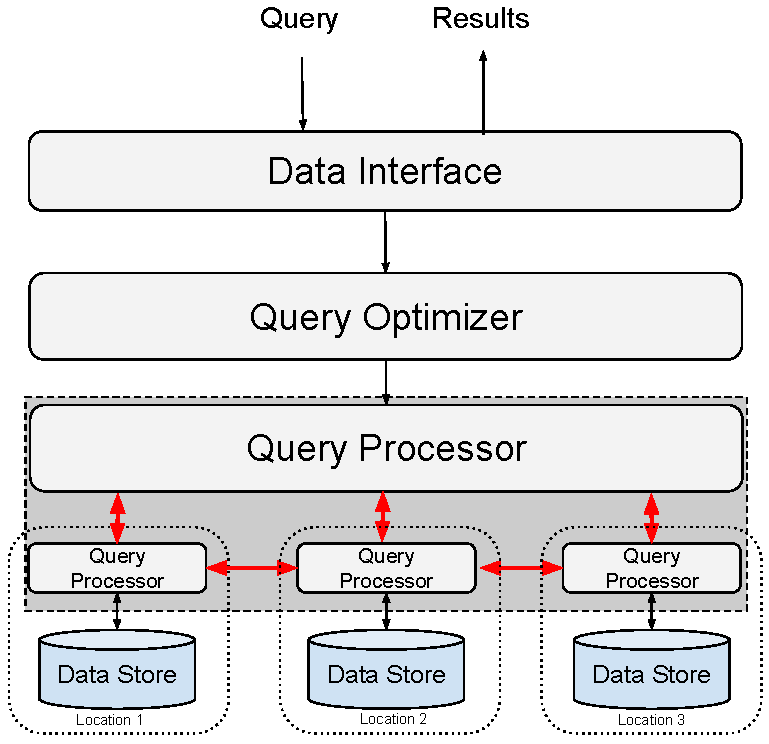
\includegraphics[width=0.35\textwidth]{figs/fdps-overview.pdf}
\caption{Federated Data Processing}
\label{fig:fdp-overview}

\end{wrapfigure}

An FDPS consists of three major components as illustrated in
Figure~\ref{fig:fdp-overview}: a data interface, a query
optimizer, and a query processor. The data interface
provides end-users (e.g., data analysts or data
administrators) the ability to query and process data that
is stored across distributed data stores in a unified
manner. The data interface upon receiving a user query
(e.g., SQL) parses and translates it into a
framework-specific internal structure (e.g., a logical query
plan). The query optimizer then rewrites the logical query
plan into a query execution plan (QEP). It extends a
single-site data processing across distributed compute
notes. To do so,  it considers communication costs between
compute nodes and introduces a global property that
describes where, i.e., at which site processing of each plan
operator happens. The query processor then ``orchestrates''
the actual execution of the query, which results in the
transfer of (intermediate) query data between compute nodes.
In geo-distributed environments, compute nodes are located
across national (or institutional) borders. In this context,
the transfer of data between sites may result in
non-compliance to data transfer regulations.



\subsection{Primer on Data Transfer Regulations} % (fold)
\label{sub:primer_on_data_transfer_regulations}

Data regulations, such as EU's General Data Protection
Regulation (GDPR)~\cite{gdpr} or California Consumer Privacy
Act (CCPA)~\cite{ccpa} significantly affect how data is
stored, processed, and transfer. In this section, we aim to
understand regulations from the perspective of data
transfers. To achieve that, we analyze GDPR articles that
regulate the transfer of data across national
borders\footnote{We note that compliance to GDPR aspects,
such as collecting, securing, storing, deleting are beyond
the scope of our current focus (see discussion in
Section~\ref{sec:related_work}).}.


GDPR articles 44--50 explicitly deal with the transfer of
data across national borders. Among these, we identified two
articles and one recital wherein the legal requirements for
transferring data fundamentally affect FDPS components.



\noindent{\bf Article~45: Transfers on the basis of an
adequacy decision.} The article dictates that transfer of
data may take place without any specific authorization,
e.g., when there is adequate data protection at the site
where data is being transferred or when data is not
subjected to regulations (i.e., when the data does not
follow the definition of personal data as in Article~4(1)).


\noindent{\bf Article~46: Transfers subject to appropriate
safeguards.} This article prescribes that (in the absence of
applicability of Article~45) data transfer can take place
under ``appropriate safeguards''. Based on the European Data
Protection Board (EDPB) recommendations that supplement
transfer tools, \emph{pseudonymisation} of data (as defined
under Article~4(5)) is considered as an effective
supplementary method.


\noindent{\bf Recital~108: Transfers under measures that
compensate lack of data protection.} Data after adequate
\emph{anonymization} (i.e., when resulting data does not
fall under Article~4(1) and as described in Recital~26) does
not fall under the ambit of GDPR and therefore can be
transferred.


\paragraph{Discussion.}Based on the above regulations, we
observe that depending on the data and to where that data is
being transferred, we can classify data transfer regulations
into:
\begin{itemize}
    \item\emph{No restrictions on transfer.} Some data
    maybe allowed to be transferred unconditionally, and
    some to only certain locations.
    \item \emph{Conditional restrictions on transfer}. For
    some data, only derived information (such as
    aggregates) or only after anonymization, can be
    transferred to (certain) locations.
    \item \emph{Complete ban on transfer}. Some data, no
    matter whatsoever, must not be transferred outside.
\end{itemize}


\subsection{Compliance by Design: Research Challenges} 
\label{sub:challenges}


Our overreaching goal is to develop methods and systems that
aid \emph{data controllers} (entities that control what data
and how the data should be processed) and \emph{data
processors} (entities that processes data on behalf of a
controller) by providing appropriate safeguards within FDPS
such that transfer---as a result of federated data
processing---of data across borders complies to regulatory
obligations described above.




\paragraph{Declarative Data Transfer Rules.}
The first and foremost challenge to achieve compliance by
design is to have declarative languages for specifying data
transfer regulations. Doing so is not trivial as regulations
affect data differently depending on its type, it's
processing, and the location where it is processed (or
transferred). For example, regulations may apply to an
entire dataset, parts of it, or even information derived
from it. Furthermore, datasets are heterogeneous in their
data models (e.g.,~graphs, relational, and textual).
Therefore, devising a declarative language where one can
specify data constraints in an easy and effective manner is
far from being simple.


\begin{wrapfigure}[13]{l}{0.4\textwidth}
\centering
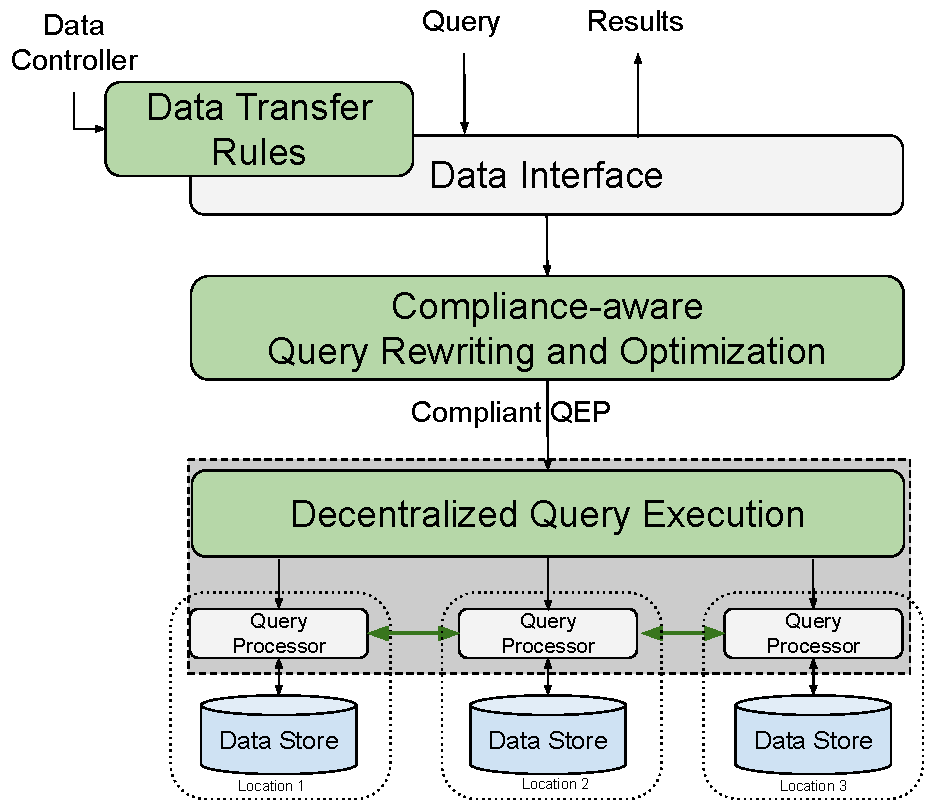
\includegraphics[width=0.35\textwidth]{figs/cbd.pdf}
\caption{Compliant FDP}
\label{fig:cbd}
\end{wrapfigure}

\paragraph{Compliance-aware Query Rewriting and
Optimization} Once a user specifies the data policies on her
data, she then needs effective and efficient ways to process
federated queries in a manner that the processing is
compliant. Achieving so is challenging as we need to extend
query rewriting and optimization capabilities. A query
optimizer should be able to transparently translate logical
query plans into compliant query execution plans by
``injecting'' operations that transform data such that the
transformed data prescribes to regulations affecting its
transfer.


\paragraph{Decentralized Query Execution} Lastly, we also
need to revisit query processors than can execute a
compliant query plan across distributed (potentially
heterogeneous) compute nodes. In contrast to current
approaches that employ a mediator-based execution, we need
meta-execution engines, which can delegate query execution
to disparate compute nodes and de-centrally execute the
query, without involving itself in the query execution.
Achieving so is crucial to make sure that data processing
happens on the locations prescribed by the query optimizer,
irrespective of the location of the processor.


\section{Compliance-aware Query Rewriting and Optimization} % (fold)
\label{sec:compliance_aware_query_rewriting_and_optimization}

We start by giving the overall idea of our approach for
achieving compliant data processing. We then discuss our
research on supporting compliance assuming relational
workloads before outlining open problems and current
research directions going beyond the relational world.




\subsection{Overall Idea}

A crucial aspect in adhering to data transfer regulations is
to transform the data in a way that renders it suitable to
be transferred across borders. From the perspective of a
FDPS, transforming (intermediate) data before shipping it to
another compute location can be considered as performing
additional \emph{masking operations} on the data. To
illustrate this, consider a two-way join query that access
data stored across Europe, North America, and Asia.
Figure~\ref{fig:overview-qo} (left) illustrates a logical
query plan for this query where orange boxes denote
cross-border operations (e.g.,~join operators) that require
inputs from two or more sources and blue circles denote
other query operators (e.g., map, filter, or aggregate). On
the right, we illustrate a corresponding execution plan,
where the optimizer decides at which site the processing of
each plan operator should happen (e.g.,~both cross-border
operators must be performed in North America). The optimizer
also rewrites the query by reordering the query operators
(e.g.,~selection pushdowns) and by ``injecting'' data
masking operators (shown by red boxes) as a means to provide
appropriate safeguards for cross-border data transfers. In
this example, both cross-border operations happen in North
America, and data from EU and Asia is transformed by a
masking operator before being shipped to North America.




\begin{figure}
  \centering
  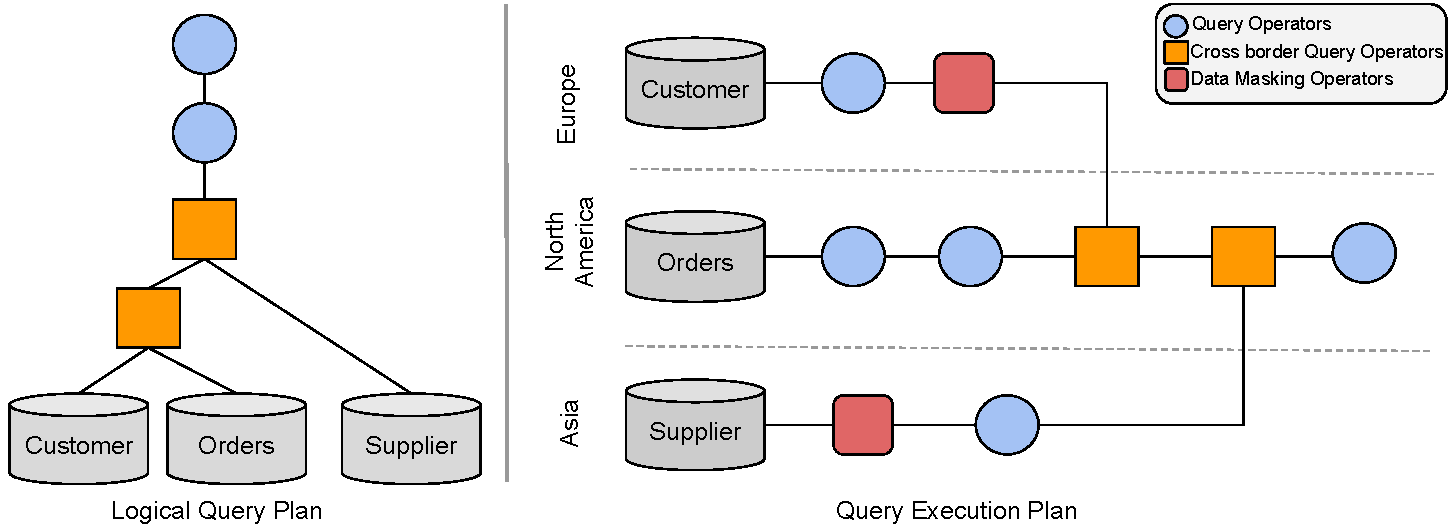
\includegraphics[scale=0.5]{figs/overview-query-optimization.pdf}
  \caption{Illustration of Query Rewriting and Optimization: (left) Logical query specified by user and (right) execution plan derived by the query optimizer after injecting masking operators.}
  \label{fig:overview-qo}
\end{figure}


\subsection{Navigating Compliance in the Relational Paradigm} % (fold)
\label{sub:current_approach}

In our current approach, we confine to processing of data
that is stored in geo-distributed SQL databases and propose
query rewriting and optimization techniques that preserve
the query semantics. In more detail, we focus on data
transfer rules that can be adhered to by data masking via
relational operations (e.g.,~project, aggregate, or filter)
such that the resulting compliant QEP retains the query
semantics, i.e.,~the output of the query should be the same
as if there were no data transfer constraints. For instance,
a projection operator can mask certain columns by projecting
them out before the (intermediate data) is transferred to
another location, and when the masked columns are not
required by the query later.

Let us illustrate this approach by expanding upon the
previous example. Consider the following schema for the
Customer, Orders, and Supplier tables along with data
transfer rules that apply to data at each
location.\\[-1.5em]

\begin{center}
\begin{tabular}{llp{0.44\textwidth}}
\toprule
\texttt{\textbf{C}ustomer} & (\textbf{c}ustkey, \textbf{n}ame, \textbf{a}cctbal, \textbf{m}ktseg, \textbf{r}egion) & Customer data can be transferred outside
    only after suppressing account balance information \\
\midrule
\texttt{\textbf{O}rders}   & (\textbf{c}ustkey, \textbf{o}rdkey, \textbf{t}otprice) & Only aggregated Orders data can be
    transferred to Asia and an order's price cannot be transferred
    to Europe \\
\midrule
\texttt{\textbf{S}upply}   & (\textbf{o}rdkey, \textbf{q}uantity, \textbf{e}xtprice) & Only aggregated Supply data for orders'
    quantity and extended price from Asia can be transferred to
    North America.\\
\bottomrule
\end{tabular} 
\end{center}


\begin{wrapfigure}[7]{r}{0.4\textwidth}
\centering
\vspace*{-0.6cm}
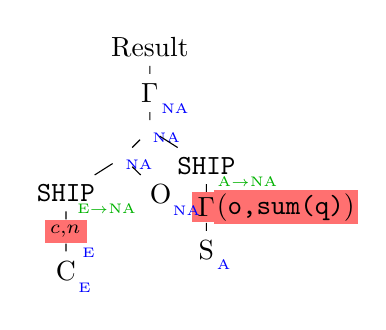
\begin{tikzpicture}
\node[] (Q) {Result};
\node[below=1mm of Q,
label={[label distance=-3mm]below right:\textcolor{blue}{\tiny{NA}}}
] (A1) {$\Gamma$};
\node[below=1mm of A1,
label={[label distance=-3mm]below right:\textcolor{blue}{\tiny{NA}}}
] (j2) {$\join$};
\node[below right=1mm and 1mm of j2,
label={[label distance=-3mm]below right:\textcolor{kgreen}{\tiny{A$\to$NA}}},
] (ship2) {\texttt{SHIP}};
\node[below = 1mm of ship2,fill=red!80!white!70, inner sep=0.7mm, 
label={[label distance=-1mm,fill=red!80!white!70, inner sep=0.4mm,]0:(\texttt{o,sum(q)})}
] (A2) {$\Gamma$};
\node[below = 1mm of A2,
label={[label distance=-3mm]below right:\textcolor{blue}{\tiny{A}}}
] (S) {S};
\node[below left=1mm and 1mm of j2,
label={[label distance=-3mm]below right:\textcolor{blue}{\tiny{NA}}}
] (j1) {$\join$};
\node[below right=1mm and 1mm of j1,
label={[label distance=-3mm]below right:\textcolor{blue}{\tiny{NA}}}
] (O) {O};
\node[below left=1mm and 1mm of j1,
label={[label distance=-3mm]below right:\textcolor{kgreen}{\tiny{E$\to$NA}}}] (ship1) {\texttt{SHIP}};
\node[below=1mm of ship1,fill=red!80!white!70, inner sep=0.7mm,
label={[label distance=-1.0mm]below right:\textcolor{blue}{\tiny{E}}}
] (proj) {$\proj_{c,n}$};
\node[below=1mm of proj,
label={[label distance=-3mm]below right:\textcolor{blue}{\tiny{E}}}] (C)  {C};


\draw[-]
(Q) -- (A1) -- (j2) -- (ship2) -- (A2) -- (S)
(j2) -- (j1) -- (O)
(j1) -- (ship1) -- (proj) -- (C)
;
\end{tikzpicture}
\end{wrapfigure}

\noindent Furthermore, consider a query $Q_{ex}$
\begin{lstlisting}[language=sql,belowskip=-15pt,aboveskip=3pt]
SELECT C.name, SUM(O.totprice), SUM(S.quantity)
FROM Customer AS C, Orders AS O, Supply AS S
WHERE C.custkey=O.custkey AND O.ordkey=S.ordkey
GROUP BY C.name
\end{lstlisting}


\noindent The query plan on the right shows a compliant QEP
as derived by our query optimizer (discussed below). Here
the \SHIP operator describes the point where intermediate
results are communicated between two sites and $\Gamma$
denotes the aggregation operator. Annotations corresponding
to each operator describe where processing of the plan
operator should happen. Observe, that executing such a plan
will not violate any of the above rules: it performs both
join operations in North America, masking data via the
projection operator $\proj_{c,n}$ suppresses the account
balance information of Customers (before the data is shipped
from Europe to North America) and via the aggregation
operator $\Gamma(\texttt{o,sum(q)})$ suppresses the orders'
quantity (prior to shipping data from Asia to North
America), as desired by the rules.


\paragraph{Policy Expression Language.}
\label{sec:policy_expressions}

One of the challenges in automatically translating
user-specified queries into compliant QEPs is to first
integrate rules into the query optimization framework. For
this, we have developed a policy expression language that
provides a simple and intuitive (SQL-like) syntax to specify
\emph{which} and \emph{where} data are allowed to be
transferred. We basically define two kinds of policy
expressions: basic and aggregate expressions. A basic
expression is of the form of a Select-Project query that can
specify restrictions pertaining to certain tables, rows,
and/or columns. An aggregate expression is of the form of a
Select-Project-GroupBy query and further allows specifying
restrictions pertaining to the transfer of aggregated
information.

\vspace{0.1cm}
\noindent\textit{Basic Expressions.} Basic expressions
allow specifying shipping of certain rows and columns of a
table to another location and have the following syntax:
\begin{expression}
  \textbf{ship} attribute list \textbf{from} table
  \textbf{to} location list \textbf{where} condition list
\end{expression}

This expression specifies cells, i.e., rows and columns, of
a table to be transferred without affecting the query
semantics.\footnote{For exposition, we restrict to
expressions over a single table. This is not a limitation:
one can specify a policy expression over more than one base
table. In this case, the condition list in the {\bf where}
clause of the expression must contain the join predicate.}
The specified cells from the table in the {\bf from} clause
(i)~belong to both columns in the {\bf ship} clause and
tuples that satisfy the predicates in the {\bf where}
clause, and (ii)~can be transferred to locations in the
\textbf{to} clause. Intuitively, if a subquery accesses only
the specified cells, then its output can be transferred to
locations specified in the expression. Consider the data
transfer rule from the above example, which does not allow
for shipping the account balance information of customers
outside Europe. Suppose the rule also allowed for shipping
customer's mktsegment and region information to North
America for commercial customers. We can use the following
two policy expressions:
  \begin{expression}
    \textbf{ship} custkey,name \textbf{from} \emph{Customer
    C} \textbf{to} \emph{Asia, North America}
  \end{expression}
\begin{expression}
  \textbf{ship} mktseg, region \textbf{from} Customer C
  \textbf{to} North America \textbf{where}
  mktseg=`commercial'
\end{expression}

\vspace{0.1cm}
\noindent\textit{Aggregate Expressions.}
For certain data, transfer rules only allow shipping of
aggregated information. For these cases, we have aggregate
expressions that allow us to specify aggregations over
columns. The syntax of an aggregate expression is given as:
\begin{expression}
  \textbf{ship} attribute list \textbf{as aggregates}
  aggregate types \textbf{from} table  \textbf{to} location
  list \textbf{where} condition list \textbf{group by}
  attribute list
\end{expression}
In the above syntax, the list of attributes in the
\textbf{ship} clause specifies cells of columns that should
be aggregated before being transferred to locations in the
location list. The \textbf{as aggregate} clause specifies
aggregation functions that should be used to aggregate
specified cells. As before, the specified cells must belong
to columns in the attribute list for the tuples that satisfy
the predicate in its \textbf{where} clause. Lastly, the
\textbf{group by} clause specifies lists of grouping
attributes for which the specified cells can be grouped by
zero, one, or more attributes from its attribute list.
Consider again the Customer data from the above example and assume
that account balance information can be transferred only after
aggregating. A possible expression is:
\begin{expression}
  \textbf{ship} acctbal \textbf{as aggregates} sum, avg
  \textbf{from} Customer C \textbf{to} * \textbf{group by}
  mktseg, region
\end{expression}

\noindent The above expression specifies how values of the
acctbal column of the Customer table can be transferred
outside. In particular, it specifies that (i)~acctbal should
be aggregated via the functions SUM or AVG and (ii)~the
cells of the acctbal column can be grouped by mktsegment
and/or by nationkey. For example, output of the queries
$\mathcal{G}_{\text{sum}(acctbal)}(C)$ and
$_{region}\mathcal{G}_{\text{avg}(acctbal)}(C) $ can be transferred
to all locations, whereas of~
$\allowbreak\mathcal{G}_{\text{sum}(acctbal)}\left(\sigma_{name=`abc'}(C)\right)$
and $\Pi_{acctbal}(C)$ cannot be transferred at all.


\paragraph{Compliance-based Optimizer.} % (fold)
\label{sec:compliance_based_optimization}
Now, in the query optimization phase, our optimizer aims to
determine if a query is legal (i.e.,~its execution does not
lead to violating data transfer rules) and to automatically
generate an optimal compliant plan. We follow a two-phase
optimization process that comprises plan annotation and site
selection. The plan annotator receives a logical plan as
input and outputs an annotated QEP. An \emph{annotated QEP}
is an optimized logical plan in which each plan operator is
annotated with a set of compliant sites (i.e., sites where
the execution of the operator will not violate any dataflow
constraint). The site selector then uses dynamic programming
to find the optimal placement of query plan operators taking
data shipping cost into account.

\begin{wrapfigure}[14]{r}{0.4\textwidth}
\small
\centering
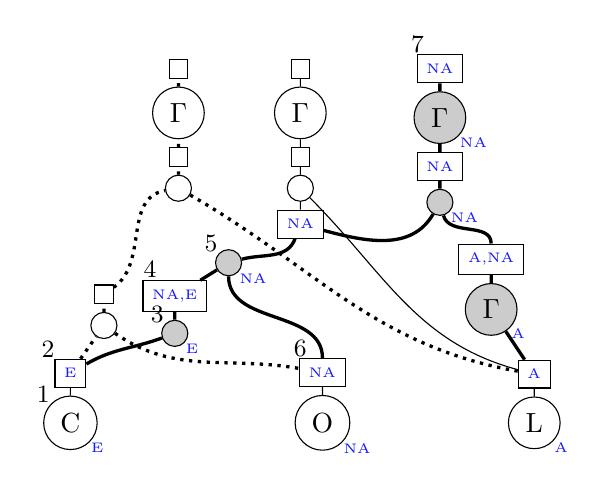
\begin{tikzpicture}
% Bottom-up construction
\node[minimum size=0.1cm,draw,label={[label distance=-1.5mm]above left:\small{1}},circle,label={[label distance=-1.5mm]below right:\textcolor{kblue}{\tiny{E}}}] (C) {C};
\node[minimum size=0.1cm,draw,circle,label={[label distance=-1.5mm]below right:\textcolor{kblue}{\tiny{NA}}},right=2.5cm of C] (O) {O};
\node[minimum size=0.1cm,draw,circle,label={[label distance=-1.5mm]below right:\textcolor{kblue}{\tiny{A}}},right=2cm of O] (L) {L};

% Relational/equivalence nodes of C,O,L
\node[minimum size=0.1cm,draw,label={[label distance=-1.5mm]above left:\small{2}}, above=0.1cm of C] (RC) {\textcolor{kblue}{\tiny{E}}};
\node[minimum size=0.1cm,draw,label={[label distance=-1.5mm]above left:\small{6}}, above=0.1cm of O] (RO) {\textcolor{kblue}{\tiny{NA}}};
\node[minimum size=0.1cm,draw, above=0.1cm of L] (RL) {\textcolor{kblue}{\tiny{A}}};

% J1
\node[minimum size=0.1cm,draw,circle,above right=0.3cm and 0.1cm of RC] (J1) {$\join$};
\node[minimum size=0.1cm,draw,above=0.1cm of J1] (EJ1) {};

% Initial path (bottom-up)
\node[minimum size=0.1cm,draw,circle,above right=1.1cm and 0.7cm of EJ1] (J2) {$\join$};
\node[minimum size=0.1cm,draw,above=0.1cm of J2] (EJ2) {};
% \node[minimum size=0.1cm,draw,circle,above=0.1cm of EJ2] (P1) {$\proj$};
% \node[minimum size=0.1cm,draw,above=0.1cm of P1] (EP1) {};
\node[minimum size=0.1cm,draw,circle,above=0.1cm of EJ2] (A1) {$\Gamma$};
\node[minimum size=0.1cm,draw,above=0.1cm of A1] (EA1) {};

% Second to left path (top-down)
\node[minimum size=0.1cm,draw,right=1.3cm of EA1] (EA2) {};
\node[minimum size=0.1cm,draw,circle,below=0.1cm of EA2] (A2) {$\Gamma$};
\node[minimum size=0.1cm,draw,below=0.1cm of A2] (EJ3) {};
\node[minimum size=0.1cm,draw,circle,below=0.1cm of EJ3] (J3) {$\join$};
\node[minimum size=0.1cm,draw,below=0.1cm of J3] (EJ4) {\textcolor{kblue}{\tiny{NA}}}; % Equiv node of left kblue join

% Blue path (top-down)
\node[minimum size=0.1cm,label={[label distance=-1.5mm]above left:\small{7}},draw,right=2.9cm of EA1] (EA1-kblue) {\textcolor{kblue}{\tiny{NA}}};
\node[minimum size=0.1cm,draw,circle,fill=gray!40,label={[label distance=-1.5mm]below right:\textcolor{kblue}{\tiny{NA}}}, below=0.1cm of EA1-kblue] (A1-kblue) {$\Gamma$};
\node[minimum size=0.1cm,draw,below=0.1cm of A1-kblue] (EJ1-kblue) {\textcolor{kblue}{\tiny{NA}}};
\node[minimum size=0.1cm,draw,circle,fill=gray!40,label={[label distance=-1.5mm]below right:\textcolor{kblue}{\tiny{NA}}}, below=0.1cm of EJ1-kblue] (J1-kblue) {$\join$};

% -- P2 (pushdown)
\node[minimum size=0.1cm,draw,fill=gray!40,label={[label distance=-1.5mm]above left:\small{3}},circle,label={[label distance=-1.5mm]below right:\textcolor{kblue}{\tiny{E}}},above right=0.2cm and 1cm of RC] (P2) {$\proj$};
% \node[minimum size=0.1cm,draw,above=0.1cm of P2] (EP2_1) {\textcolor{kblue}{\tiny{N}}};
\node[minimum size=0.1cm,label={[label distance=-1.3mm]above left:\small{4}},draw,above=0.1cm of P2] (EP2_2) {\textcolor{kblue}{\tiny{NA,E}}};
\node[minimum size=0.1cm,draw,label={[label distance=-1.5mm]above left:\small{5}},circle,fill=gray!40,label={[label distance=-1.5mm]below right:\textcolor{kblue}{\tiny{NA}}}, above right=0.1cm and 0.15cm of EP2_2] (J2-kblue) {$\join$};

% -- Aggregation (pushdown)
\node[minimum size=0.1cm,draw,circle,fill=gray!40,label={[label distance=-1.5mm]below right:\textcolor{kblue}{\tiny{A}}}, above left=0.4cm and 0.1cm of RL] (A2-kblue) {$\Gamma$};
% \node[minimum size=0.1cm,draw,above=0.1cm of A2-kblue] (EA2_1) {\textcolor{kblue}{\tiny{A}}};
\node[minimum size=0.1cm,draw,above=0.1cm of A2-kblue] (EA2_2) {\textcolor{kblue}{\tiny{A,NA}}};

% Gray Edges
\draw[-]
(C) -- (RC)
(O) -- (RO)
(L) -- (RL)

(RL) to[out=165,in=-45] (J3)
(EA2) -- (A2) -- (EJ3) -- (J3) -- (EJ4)
;

% Initial plan (dotted lines)
\draw[dotted,very thick,-]
(RC) -- (J1) to[out=-35,in=170] (RO) 
(J1) -- (EJ1) to[out=35,in=190] (J2)
(J2) -- (EJ2) -- (A1) -- (EA1)
(RL) to[out=170,in=-30] (J2)

;

% Compliant Edges
\draw[very thick,-]
(EA1-kblue) -- (A1-kblue) -- (EJ1-kblue) -- (J1-kblue)
(RC) to[out=30,in=200] (P2)
(P2) -- (EP2_2)
(EP2_2) -- (J2-kblue)
(J2-kblue) to[out=15,in=250] (EJ4)
(EJ4) to[out=-15,in=240] (J1-kblue)
(EA2_2) to[out=90,in=-75] (J1-kblue)
(RL) -- (A2-kblue) -- (EA2_2)
(RO) to[out=90,in=-90] (J2-kblue)
;

\end{tikzpicture}
% \caption{Simplified search space for $Q_{ex}$.}
% \label{fig:search_space}
\end{wrapfigure}

More specifically, we adapt the Volcano optimizer
generator~\cite{GraefeM93} to generate the plan annotator.
Our adaptations allow us to produce an annotated plan by
enumerating the plan space by applying algebraic equivalence
rules in a top-down fashion and filter compliant ones by
applying our annotation rules in a bottom-up fashion. To do
so, we treat geo-locations associated with base tables as
``interesting properties'' and propagate these properties
bottom-up via annotation rules. Our annotation rules are
based on the structure of the subplans and make use of a
lightweight mechanism to evaluate data transfer rules. Our
policy evaluator allows for easy integration of policy
expressions into the annotation process. In particular,
during plan enumeration, it determines to which
cross-borders sites the output of operators can be shipped.
The figure on the right illustrates the annotation process
for our running example. Here the plan with the dotted lines
shows the initial logical plan. The plan with thick solid
lines shows the annotated plan which the annotator outputs.
The letters in the square boxes denote sites to which the
output of an operator can be shipped to and letters below
each operator denote sites where each plan operator can be
executed. For example, the project operator (node~3) must be
executed in Europe but its output (node~4) can be shipped to
North America and Europe. It is easy to see that the plan
with thick solid lines translates to the compliant plan
shown above. For a more detailed description of our
optimizer, we refer readers to \cite{cqp-sigmod}, which also
gives a more formal treatment and proof of correctness.




% subsection current_approach (end)



\subsection{Compliance Beyond the Relational Paradigm} % (fold)
\label{sub:open_problems_&_research_directions}

Data masking via relational operations and our above query
rewriting and optimization techniques have inherent
limitations. They limit the whole gamut of compliant QEPs.
As conditional restrictions on data transfers (as discussed
in Section~\ref{sub:primer_on_data_transfer_regulations})
may allow transferring of pseudonymized and/or anonymized
data, it is important to expand the scope of masking
functions to beyond relational operations.


\paragraph{Advanced Masking Functions.} Based on European
Commission's Opinions on Anonymization
Techniques~\cite{eu-dpw}, we consider the following masking
operations in addition\footnote{We note that this is not an
exhaustive list of masking functions that we plan to
support}.
\begin{center}
\begin{tabular}{l>{\em}p{140mm}}
\toprule
Masking function & Description \\
\midrule
Suppression      & Similar to Projecting out, replaces a value with a generic value (e.g.,~`xxx') \\
Pseudonymisation & Replaces one value with another, s.t., new value has no logical relationship to the original (e.g., `abc' $to$ 'xyz')  \\
Blurring         & Alters a value by partial suppression (e.g.,~`abc' $\to$ 'aXX') \\
Generalization   & Generalizes a value using a predefined domain hierarchy (e.g.,~`23' $\to$ `20--25') \\
Shuffling        & Replaces existing values with values from the same column\\
Noise Addition   & Alter accuracy of (numeric) attributes\\
\bottomrule  
\end{tabular}
\end{center}


\emph{Interleaving masking operators with query operators.}
A direct consequence of masking via non-relational
operations is that: (1)~it may no longer be possible to
preserve query semantics. To illustrate this, consider that
when transferring employee records, the age attribute is
generalized by a function $f$ that translates numeric
attributes to certain range intervals (e.g., $f(23)=20-25$).
Such a masking may change the data type (e.g., \texttt{int}
to \texttt{int4range}) leading to change in query semantics.
As another example, now consider that the age attribute is
masked via suppression. In this case too, the resulting
records will contain fewer attributes than that desired by
the query. (2)~Naive interleaving may affect robustness of
the data masking. For example, consider a masking function
$f$ that blurs zipcode (e.g., $f(12345)=123\text{xx}$). In
this case a filter predicate $p$ on zipcode (e.g., $p\equiv$
zipcode=12345) evaluated before masking may lead to possible
singling out of an individual records. To this end, our
current work explores the following research questions.

\begin{itemize}
  \item[Q1] \emph{How to interpose masking functions with
  query operators such that the resulting data is still
  anonymized?} For example, for scalar and univariate
  masking functions (e.g.,~blurring), we can substitute
  filter predicate by an UDF filter where the UDF is the
  masking function (e.g., we can rewrite $p$ as zipcode=$f(12345)$.
  \item[Q2] \emph{How to minimize information loss by
  ``injecting'' the right masking functions?} For example,
  by exploiting the fact that noise addition preserves
  aggregates (such as SUM() and AVG()), we can use masking
  via noise addition for aggregate queries instead of
  masking by blurring.
\end{itemize}

 
\paragraph{General Purpose Dataflow Programs.} Many data
analytics tasks are expressed as directed (a)cyclic graphs
(DAG) composed of second order functions (e.g.,~map). To
this end, we are investigating how advanced masking function
can be composed with dataflow operators. For this, we plan
to leverage our prior work on dataflow
optimizations~\cite{heuske2012} and investigate effective
and efficient ways to support (iterative) DAG programs.



\section{Decentralized Query Execution} % (fold)
\label{sec:decentralized_query_execution}

We now turn our attention to the execution of compliant
QEPs. We first discuss why current FDPS fall short of
executing compliant QEPs. We then present key challenges we
need to tackle before presenting our approach.


\begin{wrapfigure}[10]{r}{0.4\textwidth}
\centering
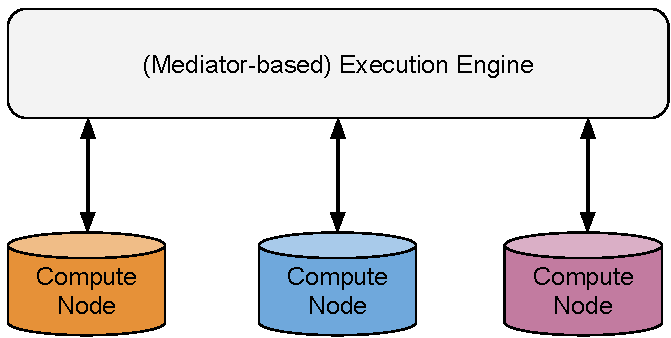
\includegraphics[width=0.35\textwidth]{figs/mediator-based.pdf}
\caption{Centralized FDP}
\end{wrapfigure}

\paragraph{State-of-the-art \& Limitations.}
State-of-the-art FDPS (such as Presto~\cite{presto}) mostly
follow a mediator-based
approach~\cite{Josifovski:2002:GNF:564691.564751}. Although,
such an approach (as illustrated by the figure on the right)
is useful for performing data analytics across heterogeneous
compute nodes, it does not lend itself to executing
compliant QEPs. This is because \emph{cross-database
operations} (i.e., operators requiring inputs from multiple
databases) are performed by the mediator's execution engine.
This leads to the added complexity in ensuring compliance
(due to the centralized processing by the mediator) to data
transfers during query execution. To see this, recall the
example of Section~\ref{sub:current_approach}, and consider
that now Orders data from North America can be transferred
to Asia but nothing can move out from Asia. Under these
constraints, a possible compliant plan is to first ship the
data (after masking via projection operator as before) from
Europe to North America, perform the first cross-database
operation ($R\equiv C\join O$) in Europe, and the second
cross-database operation ($R \join S$) in Asia. Current FDPS
cannot execute such multi-site queries. Another limitation
arises when metadata (or statistics) cannot be freely shared
across sites, which leads to bad QEPs.


\paragraph{Challenges.} In contrast to mediator-based
approaches, we need a fully-decentralized approach
(i.e.,~without any central entity in the execution pipeline)
to execute queries over geo-distributed compute nodes. This,
however, poses several challenges:

\begin{enumerate}
  \item System Interoperability: A key aspect in achieving
  a fully-decentralized query execution is the ability to
  communicate (intermediate) data between underlying data
  processing systems. A key challenge, therefore, is to make
  systems interoperable without affecting their autonomy,
  even without them noticing.

 \item Fast Data Transfer: As a consequence of lack of
systems' interoperability, moving data among different data
processing systems incur a high cost (e.g.,~we might need to
export data from one DBMS and import that data in another
DBMS). The challenge resides in enabling ``native'' data
transfers (e.g.,~reading a relation from a DBMS directly
from its binary store) without affecting the autonomy of the
underlying processing systems.

\item Incompatible Data Formats: Different systems work on
different internal data formats, which adds additional
complexity and non-trivial cost of storing and converting
data from one format to another during data transfers. The
main question to answer is: does an intermediate data
representation exists that can speed up the conversion from
any source data format to any target data format?

\item Query Optimization: Last but not the least,
optimizing queries without having a ``centralized'' access
to data systems makes query optimization across
geo-distributed data processing systems non-trivial. For
example, data processing systems have their own cost models,
which impedes in determining global cost of executing
queries.

\end{enumerate}



\begin{wrapfigure}[14]{r}{0.4\textwidth}
\centering
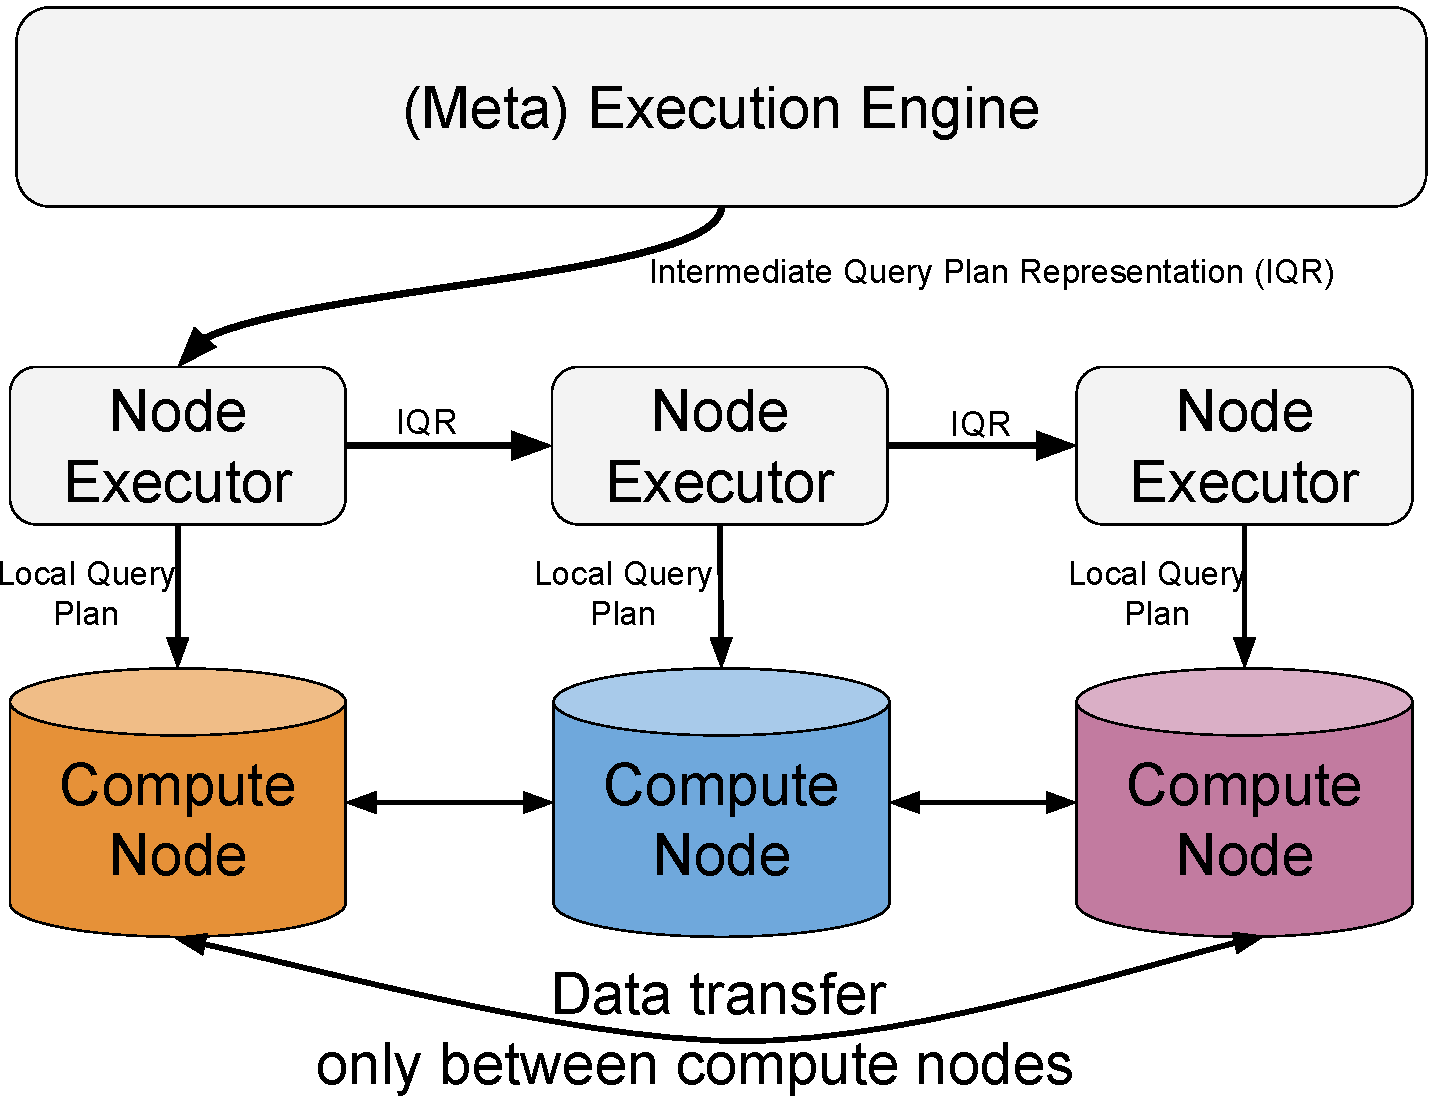
\includegraphics[width=0.35\textwidth]{figs/delegator-based.pdf}
\caption{Decentralized FDP}
\label{fig:delegator-based}
\end{wrapfigure}

\paragraph{Our Approach.} We have
developed a meta-execution engine, which enables executing
federated queries in a decentralized fashion.
Figure~\ref{fig:delegator-based} illustrates our overall
approach. In contrast to a mediator-based approach, we
follow what we refer to as a delegator-based approach. The
Meta-execution engine, delegates the entire query execution
to underlying data processing systems. This avoids a need to
have any central entity in the execution pipeline, and data
transfer only happens among compute nodes following
annotations as prescribed by the compliance-aware query
optimizer.

In more detail, the meta execution engine first globally
optimizes a query (with limited available metadata) and
translates the plan into an intermediate representation
(IQR). The IQR is agnostic to underlying data processing
platforms and encapsulates query semantics comprising local
subplans (i.e., processing that should be limited to certain
locations) and inter-operator (cross-database) communication
endpoints as well as mechanics of data movement between
different systems. The node executors are local meta
execution engines that are responsible for (a)~translating
and optimizing a local-subplan into platform specific query
plan (e.g., to a Spark program), (b)~communicating the IQR
to other (relevant) node executors, and (c)~facilitating the
data movement between systems either by leveraging
underlying system's capabilities (see below) or by creating
suitable data ``pipes''. It is important to note that the
node executors themselves do not execute any part of the
query but only delegate execution to underlying systems.



In our current prototype~\cite{cqp-vldb}, we support such
decentralized query execution over multiple RDBMSes
(including PostgreSql, MariaDB, MySQL, Hive, and DB2). To do
so, the local node executors leverage the SQL/MED standard
to communicate intermediate query data between systems. More
specifically, while translating into a local DBMS specific
program, the node executor first registers external tables
(i.e., tables corresponding to the output of remote
subplans) as local tables. This enables achieving a
completely decentralized query execution.



\paragraph{Current Research Directions.} We are currently 
investigating how to process data using geo-distributed
heterogeneous compute platforms. For example, how can we
execute a multi-site query using a PostgreSql database at
one site and a Spark Cluster at another site? This is
crucial to support compliance for non-relational workloads.
To this end, our work includes expanding capabilities of
cross-platform data processing systems (such as Apache
Wayang~\cite{rheem}) to support geo-distributed compute
sites. We are also investigating suitable common data
formats such as Parquet, Protocol Buffers, or Avro, which
makes inter-system data transfers efficient.



\section{Related Work} % (fold)
\label{sec:related_work}

We now relate the ideas presented in this paper to prior
work on compliance and federated data processing.

\noindent{\bf Compliance.} With growing concerns over data
privacy and enforcement of regulations, several works have
looked into various legal contexts within with data
processing systems must be designed. With respect to GDPR
compliance, most works have focused on data subjects' rights
as a large proportion of GDPR governs data storage. In this
regard, \cite{Mohan2019} analyzed various aspects of GDPR
including deletion, indexing, monitoring and logging, and
access control, and how they impact database systems.
\cite{GDPRBench, Shastri2020} studied the performance of
GDPR compliant systems. Their work mainly considers rights
of data subjects (e.g., customers) and provide a benchmark
to evaluate data processing aspects including metadata
indexing, deletion, access control, and encryption.
\cite{Kraska2019,Kraska2019SchengenDB} proposed an
architectural vision for a database that natively supports
auditing, deletion, and user consent management.
\cite{shastri2019gdpr} and \cite{Shastri19-hotcloud} examine
how GDPR affects the design and operation of modern
computing systems. \cite{Schwarzkopf2019} and
\cite{wang2019-datacapsule} studied supporting restrictions
based on ``purpose''-based access control. \cite{shah2019}
presents an analysis on the impact of GDPR on storage
systems. \cite{zsolt2021-sdp} presents a vision for
Software-Defined Data Protection, for which they propose
leveraging recent advances in Software-Defined Storage
(e.g., FPGA-based key-value stores) to achieve compliance at
the storage level. In the context of dataflow processing,
\cite{spenger2021} investigated supporting of data subject's
privacy request (for access, deletion, and objection) by
adopting causal snapshot consistency. \cite{arfelt2019}
focuses on auditing GDPR compliance based on logs. All the
above work can be seen as complementary to our work. While
the aforementioned works focus more on data subject's
rights, we focus more on the actual processing of the data
wherein we consider regulations pertaining to the movement
of data. Perhaps, closest to our work on compliance-aware
query optimization is that of \cite{guido2019} and
\cite{Farnan2014,Farnan2013}. While these works only focus
on the operator placement problem based on privacy or
user-specified constraints, we additionally consider
rewriting queries by extending and interleaving query
operators with data masking functions.


\noindent{\bf Federated Data Processing.} Our work is also
related to earlier works on multi-database query
processing~\cite{1Kossmann2000} and more recent work on
cross-platform systems~\cite{rheem} and
polystores~\cite{bigdawg2015}. It differs from the former in
that we focus on heterogeneous compute infrastructures and
from the latter in that we target geo-distributed
environments and a facilitate a  decentralized query
execution.







% section related_work (end)
\section{Conclusion}

Growing concerns on data privacy and usage preclude data
transfers across national (or organizational) borders. It is
therefore crucial that data processing in federated
environments be compliant with data transfer regulations. In
this paper, we have analyzed data transfer regulations from
the perspective of GDPR and discussed key research
challenges for including compliance aspects in federated
data processing. We presented our approach for compliant
geo-distributed data processing that focuses on relational
workloads. We also discussed how query rewriting and
optimization techniques must be extended to support data
masking and outlined open problems and research directions
to support workloads beyond relational workloads. We have
advocated the need for decentrally executing queries and
presented challenges and research directions to support data
analytics over geo-distributed and heterogeneous compute
infrastructures.



\paragraph{Acknowledgements}
This work is funded by the German Ministry for Education \&
Research as BIFOLD – ``Berlin Institute for the Foundations
of Learning and Data'' (01IS18025A and 01IS18037A).


\begin{thebibliography}{10}
\itemsep=1pt
\begin{small}


\bibitem{gdpr}
Regulation (eu) 2016/679 of the European parliament and of the council of 27
  april 2016 on the protection of natural persons with regard to the processing
  of personal data and on the free movement of such data, and repealing
  directive 95/46. \newblock 59:1--88, 2016.


\bibitem{ccpa}
California consumer privacy act. California civil code, section 1798.100, June 28. 
\newblock 2018.



\bibitem{rheem}
Divy Agrawal, Sanjay Chawla, Bertty Contreras-Rojas, Ahmed Elmagarmid, Yasser
  Idris, Zoi Kaoudi, Sebastian Kruse, Ji~Lucas, Essam Mansour, Mourad Ouzzani,
  Paolo Papotti, Jorge-Arnulfo Quian\'{e}-Ruiz, Nan Tang, Saravanan
  Thirumuruganathan, and Anis Troudi.
\newblock Rheem: Enabling cross-platform data processing: May the big data be
  with you!
\newblock \emph{Proc. VLDB Endow.}, 11 (11): 1414–1427,
  2018.

\bibitem{arfelt2019}
Debois~S. Arfelt~E., Basin~D.
\newblock Monitoring the {GDPR}.
\newblock In \emph{ESORICS}, pages 681--699, 2019.

\bibitem{cqp-vldb}
Kaustubh Beedkar, David Brekardin, Jorge-Anulfo Quian\'{e}-Ruiz, and Volker
  Markl.
\newblock Compliant geo-distributed data processing in action.
\newblock \emph{Proc. VLDB Endow.}, 14 (12): 2843–2846,
  2021.

\bibitem{cqp-sigmod}
Kaustubh Beedkar, Jorge-Arnulfo Quian\'{e}-Ruiz, and Volker Markl.
\newblock Compliant geo-distributed query processing.
\newblock In \emph{ACM SIGMOD}, page 181–193, 2021.

\bibitem{bigdawg2015}
Jennie Duggan, Aaron~J. Elmore, Michael Stonebraker, Magda Balazinska, Bill
  Howe, Jeremy Kepner, Sam Madden, David Maier, Tim Mattson, and Stan Zdonik.
\newblock The bigdawg polystore system.
\newblock \emph{SIGMOD Rec.}, 44 (2): 11–16, 2015.

\bibitem{Farnan2013}
Nicholas~L. Farnan, Adam~J. Lee, Panos~K. Chrysanthis, and Ting Yu.
\newblock {PAQO}: A preference-aware query optimizer for postgresql.
\newblock \emph{Proc. VLDB Endow.}, 6 (12): 1334–1337,
  2013.

\bibitem{Farnan2014}
Nicholas~L. Farnan, Adam~J. Lee, Panos~K. Chrysanthis, and Ting Yu.
\newblock {PAQO}: Preference-aware query optimization for decentralized
  database systems.
\newblock pages 424--435, 2014.

\bibitem{cms-gdpr-fines}
GDPR Enforcement Tracker.
\newblock \url{https://www.enforcementtracker.com/}.

\bibitem{GDPRBench}
G{D}{P}{R}bench.
\newblock \url{https://www.gdprbench.org/gdpr}.

\bibitem{GraefeM93}
Goetz Graefe and William~J. McKenna.
\newblock The volcano optimizer generator: Extensibility and efficient search.
\newblock In \emph{ICDE}, pages 209--218, 1993.

\bibitem{heuske2012}
Fabian Hueske, Mathias Peters, Matthias~J. Sax, Astrid Rheinl\"{a}nder, Rico
  Bergmann, Aljoscha Krettek, and Kostas Tzoumas.
\newblock Opening the black boxes in data flow optimization.
\newblock \emph{Proc. VLDB Endow.}, 5 (11): 1256–1267,
  2012.

\bibitem{Hung2015}
Chien-Chun Hung, Leana Golubchik, and Minlan Yu.
\newblock Scheduling jobs across geo-distributed datacenters.
\newblock In \emph{SoCC}, page 111–124, 2015.

\bibitem{zsolt2021-sdp}
Zsolt Istv\'{a}n, Soujanya Ponnapalli, and Vijay Chidambaram.
\newblock Software-defined data protection: Low overhead policy compliance at
  the storage layer is within reach!
\newblock \emph{Proc. VLDB Endow.}, 14 (7): 1167–1174,
  2021.

\bibitem{Josifovski:2002:GNF:564691.564751}
Vanja Josifovski, Peter Schwarz, Laura Haas, and Eileen Lin.
\newblock Garlic: A new flavor of federated query processing for db2.
\newblock In \emph{SIGMOD}, pages 524--532, 2002.

\bibitem{1Kossmann2000}
Donald Kossmann.
\newblock The state of the art in distributed query processing.
\newblock \emph{ACM Comput. Surv.}, 32 (4): 422–469, 2000.

\bibitem{Kraska2019SchengenDB}
Tim Kraska, Michael Stonebraker, Michael Brodie, Sacha Servan-Schreiber, and
  Daniel Weitzner.
\newblock \emph{SchengenDB: A Data Protection Database Proposal}, pages 24--38.
\newblock 2019.

\bibitem{Kraska2019}
Tim Kraska, Michael Stonebraker, Michael Brodie, Sacha Servan-Schreiber, and
  Daniel~J. Weitzner.
\newblock Datumdb: A data protection database proposal.
\newblock In \emph{Poly'19 co-located at VLDB 2019}, 2019.

\bibitem{Mohan2019}
Jayashree Mohan, Melissa Wasserman, and Vijay Chidambaram.
\newblock Analyzing gdpr compliance through the lens of privacy policy.
\newblock In Vijay Gadepally, Timothy Mattson, Michael Stonebraker, Fusheng
  Wang, Gang Luo, Yanhui Laing, and Alevtina Dubovitskaya, editors,
  \emph{Poly'19 co-located at VLDB 2019}, 2019.

\bibitem{eu-dpw}
Opinion 05/2014 on Anonymisation Techniques.
\newblock
  \url{https://ec.europa.eu/justice/article-29/documentation/opinion-recommendation/files/2014/wp216\_en.pdf}.

\bibitem{Pu:2015}
Qifan Pu, Ganesh Ananthanarayanan, Peter Bodik, Srikanth Kandula, Aditya
  Akella, Paramvir Bahl, and Ion Stoica.
\newblock Low latency geo-distributed data analytics.
\newblock In \emph{SIGCOMM}, pages 421--434, 2015.

\bibitem{guido2019}
Guido Salvaneschi, Mirko K\"{o}hler, Daniel Sokolowski, Philipp Haller,
  Sebastian Erdweg, and Mira Mezini.
\newblock Language-integrated privacy-aware distributed queries.
\newblock \emph{Proc. ACM Program. Lang.}, 3 (OOPSLA), 2019.

\bibitem{Schwarzkopf2019}
Malte Schwarzkopf, Eddie Kohler, M.~Frans Kaashoek, and Robert Morris.
\newblock Position: {GDPR} compliance by construction.
\newblock In \emph{Poly'19 co-located at VLDB 2019}, 2019.

\bibitem{presto}
Raghav Sethi, Martin Traverso, Dain Sundstrom, David Phillips, Wenlei Xie,
  Yutian Sun, Nezih Yegitbasi, Haozhun Jin, Eric Hwang, Nileema Shingte, and
  Christopher Berner.
\newblock Presto: Sql on everything.
\newblock In \emph{ICDE}, pages 1802--1813, 2019.

\bibitem{shah2019}
Aashaka Shah, Vinay Banakar, Supreeth Shastri, Melissa Wasserman, and Vijay
  Chidambaram.
\newblock Analyzing the impact of {GDPR} on storage systems.
\newblock In \emph{USENIX Workshop on Hot Topics in Storage and File Systems
  (HotStorage 19)}, 2019.

\bibitem{Shastri19-hotcloud}
Supreeth Shastri, Melissa Wasserman, and Vijay Chidambaram.
\newblock The seven sins of {Personal-Data} processing systems under {GDPR}.
\newblock In \emph{USENIX Workshop on Hot Topics in Cloud Computing (HotCloud
  19)}, 2019.

\bibitem{shastri2019gdpr}
Supreeth Shastri, Melissa Wasserman, and Vijay Chidambaram.
\newblock Gdpr anti-patterns: How design and operation of modern cloud-scale
  systems conflict with gdpr, 2019.

\bibitem{Shastri2020}
Supreeth Shastri, Vinay Banakar, Melissa Wasserman, Arun Kumar, and Vijay
  Chidambaram.
\newblock Understanding and benchmarking the impact of gdpr on database
  systems.
\newblock \emph{Proc. VLDB Endow.}, 13 (7): 1064–1077,
  2020.

\bibitem{spenger2021}
Jonas Spenger, Paris Carbone, and Philipp Haller.
\newblock Wip: Pods: Privacy compliant scalable decentralized data services.
\newblock In \emph{Poly 2021 and DMAH 2021}, page 70–82, 2021.

\bibitem{Taft2020}
Rebecca Taft, Irfan Sharif, Andrei Matei, Nathan VanBenschoten, Jordan Lewis,
  Tobias Grieger, Kai Niemi, Andy Woods, Anne Birzin, Raphael Poss, Paul
  Bardea, Amruta Ranade, Ben Darnell, Bram Gruneir, Justin Jaffray, Lucy Zhang,
  and Peter Mattis.
\newblock Cockroachdb: The resilient geo-distributed sql database.
\newblock In \emph{ACM SIGMOD}, page 1493–1509, 2020.

\bibitem{agora}
Jonas Traub, Zoi Kaoudi, Jorge-Arnulfo Quian\'{e}-Ruiz, and Volker Markl.
\newblock Agora: Bringing together datasets, algorithms, models and more in a
  unified ecosystem [vision].
\newblock \emph{SIGMOD Rec.}, 49 (4): 6–11, 2021.

\bibitem{Vulimiri:2015}
Ashish Vulimiri, Carlo Curino, Brighten Godfrey, Konstantinos Karanasos, and
  George Varghese.
\newblock Wanalytics: Analytics for a geo-distributed data-intensive world.
\newblock In \emph{CIDR}, 2015.

\bibitem{wang2019-datacapsule}
Lun Wang, Joseph~P. Near, Neel Somani, Peng Gao, Andrew Low, David Dao, and
  Dawn Song.
\newblock Data capsule: {A} new paradigm for automatic compliance with data
  privacy regulations.
\newblock \emph{CoRR}, abs/1909.00077, 2019.



\end{small}
\end{thebibliography}

\end{document}
